% !TeX program = xelatex
% 编译：xelatex 典型的信号.tex（VS Code 的 LaTeX Workshop 会读上一行，自动用 xelatex）
% 来源：2022 浙江大学《信号与系统》胡浩基老师，第 1 章前两节课（视频约 59 分钟）。
\documentclass[UTF8,a4paper,11pt]{ctexart}
\usepackage{amsmath,amssymb}
\usepackage{geometry}
\geometry{margin=2.4cm}
\usepackage{xcolor}
\usepackage{mdframed}
\usepackage{booktabs}
\usepackage{enumitem}
\usepackage{tikz}
\usepackage{float}

\setCJKmainfont{Songti SC}[BoldFont={Songti SC Bold}]
\setCJKsansfont{PingFang SC}

\newmdenv[backgroundcolor=blue!4,linecolor=blue!50!black,linewidth=1pt,innertopmargin=6pt,innerbottommargin=6pt]{rememberbox}
\newenvironment{remember}{\begin{rememberbox}\textbf{必须背下来}\par\smallskip}{\end{rememberbox}}
\newmdenv[backgroundcolor=yellow!8,linecolor=orange!70!black,linewidth=1pt,innertopmargin=6pt,innerbottommargin=6pt]{notebox}
\newenvironment{note}{\begin{notebox}\textbf{说明}\par\smallskip}{\end{notebox}}
\newcommand{\Sa}{\operatorname{Sa}}
\renewcommand{\d}{\,\mathrm{d}}

\title{典型的信号\\\large 浙江大学 2022《信号与系统》（胡浩基）第 1 章 听课笔记}
\author{}
\date{}

\begin{document}
\maketitle

\begin{note}
这份笔记由视频整理而来，来源要分清：
\begin{itemize}[nosep]
\item 概念与口述内容：来自语音转写。转写模型很小，错字很多（如「阶跃」被写成「接越」），我按上下文还原；
\item 板书公式与证明：来自画面。第一遍转写的 41:30--54:30 一段因 whisper 复读而失效，后来换用 large-v3-turbo 模型（关闭上下文、加术语提示词）对 40:00--56:00 重新转写，这一段已基本恢复；证明的步骤我用重转写的讲解与板书截图互相对照过；
\item 标注「（补充）」的内容是我自己加的，课上没讲，或讲了但我没听清。
\end{itemize}
\end{note}

\section{一句话主干}
本节讲的是：\textbf{信号怎么分类}，以及\textbf{后面整门课都会反复用到的四个基本信号}——阶跃(unit step)、冲激(impulse)、抽样函数(sampling function)，外加离散里对应的单位脉冲和单位阶跃。其中有两个「必须记住的积分结果」，后面推傅里叶变换要用。

%==================================================================
\section{信号与系统是什么}
\begin{itemize}
\item \textbf{信号}(signal)：表达、传递信息的符号。
\item \textbf{系统}(system)：有输入、有输出。接收一个输入信号，处理之后变成另一个信号输出。
\end{itemize}

%==================================================================
\section{信号的分类}
老师说：书上第 3 页起有很多分类，只讲重要的，有时还会自己加一个。第一个「按维度分」就是他自己加的，不在书上。

\subsection{按维度分：这门课只讨论一维}
\begin{tabular}{@{}lll@{}}
\toprule
维度 & 例子 & 自变量 $\to$ 取值 \\
\midrule
一维 & 声音（语音）信号 & 时间 $\to$ 声音强度 \\
二维 & 图像 & （横坐标，纵坐标）$\to$ RGB 三个数 \\
三维 & 视频；深度图 & 图像两个维度 $+$ 时间；图像两个维度 $+$ 深度 \\
四维 & VR 眼镜看到的画面 & 三维 $+$ 时间 \\
\bottomrule
\end{tabular}

\medskip
老师的几个说法：
\begin{itemize}[nosep]
\item 图像里每个点用 RGB 三个数编码，按课上的说法每个数用 24 比特（取值 $0\sim 2^{24}-1$）。\emph{（补充：两次独立转写（base 与 large-v3-turbo）都是这个说法，所以这是老师原话，不是听错。但与常见事实不符：常见做法是红、绿、蓝\textbf{三个通道各 8 比特，合起来一个像素 24 比特}，取值 $0\sim255$。老师这里很可能是把「一个像素的总比特数」说成了「每个数的比特数」。这属于口误，对后面的内容没有影响，以 8 比特/通道为准，我没有核对书。）}
\item 人看到一幅图像，计算机看到的是三个矩阵（红、绿、蓝各一个）。
\item 视频的帧率：传统 24 帧，高清 50 帧。
\item \textbf{只讨论一维}，原因是简单：一维是学二、三、四维的基础，不是高维不重要，而是它们在别的课里学。二维傅里叶变换会给公式，但不展开。
\end{itemize}

\subsection{连续信号与离散信号}
\begin{remember}
\begin{center}
圆括号 $x(t)$ $\Rightarrow$ 连续信号，$t\in\mathbb{R}$\qquad\qquad
方括号 $x[n]$ $\Rightarrow$ 离散信号，$n\in\mathbb{Z}$
\end{center}
整本书统一这个写法，\textbf{没有 $x[t]$，也没有 $x(n)$}。老师特别提醒：学到后面做离散傅里叶变换，明明写的是方括号，做着做着套回连续的公式，是常见的错。
\end{remember}

学生问过：为什么 $n$ 只能取整数，不能取 $0.5$？老师的回答：$n$ 只是一个「名字」，只表示「我不在实数轴上取值，而在一个离散的集合上取值」；用 $-0.5,0.5$ 当名字也行，但为了统一，约定用整数。

\subsection{周期信号与非周期信号}
\textbf{连续}：
\[
x(t)=x(t+mT),\quad m\in\mathbb{Z}
\]
$T$ 取\textbf{最小正周期}。若 $T$ 是周期，则 $2T,3T,\dots$ 也都是周期，其中最小的正的那个叫基本周期。

\textbf{离散}：
\[
x[n]=x[n+mN],\quad m\in\mathbb{Z},\ N\ \text{为正整数}
\]
老师口述这里的 $N$ 是「自然数」，我写成正整数是因为 $N=0$ 时「重复」没有意义。老师的教学要求：「举一反三、触类旁通」。以后他有时只给连续或只给离散的定义，另一个要自己补出来。

\subsection{奇信号与偶信号}
\begin{align*}
\text{偶信号}\ (\text{even}):&\quad x(t)=x(-t)\quad \text{关于纵轴对称}\\
\text{奇信号}\ (\text{odd}):&\quad x(t)=-x(-t)\quad \text{关于原点旋转 }180^\circ\text{ 对称}
\end{align*}
老师评价：这就是高中的奇函数、偶函数，不算本课新知识。

\subsubsection*{本课第一个真正的新知识：任何信号都能唯一分解成「偶 $+$ 奇」}
\begin{remember}
\textbf{定理。}对任意信号 $x(t)$（定义域关于原点对称，如 $t\in\mathbb{R}$），存在\textbf{唯一}的一对信号 $x_e(t)$、$x_o(t)$，其中 $x_e$ 是偶信号、$x_o$ 是奇信号，使得
\[
x(t)=x_e(t)+x_o(t),\qquad\text{并且}\quad
x_e(t)=\frac{x(t)+x(-t)}{2},\quad x_o(t)=\frac{x(t)-x(-t)}{2}.
\]
\end{remember}
这里 $e$ 是 even，$o$ 是 odd，下标是这么来的。要证明的有两件事：\textbf{存在}（至少有一种拆法）和\textbf{唯一}（至多有一种拆法）。

\paragraph{证明一：存在性。}直接把上面的 $x_e,x_o$ 定义出来，验三条：
\begin{enumerate}[nosep]
\item \textbf{$x_e$ 是偶的}：
$x_e(-t)=\dfrac{x(-t)+x\bigl(-(-t)\bigr)}{2}=\dfrac{x(-t)+x(t)}{2}=x_e(t)$。
\item \textbf{$x_o$ 是奇的}：
$x_o(-t)=\dfrac{x(-t)-x(t)}{2}=-\dfrac{x(t)-x(-t)}{2}=-x_o(t)$。
\item \textbf{加起来是 $x(t)$}：
$x_e(t)+x_o(t)=\dfrac{x(t)+x(-t)+x(t)-x(-t)}{2}=\dfrac{2x(t)}{2}=x(t)$。
\end{enumerate}
三条都成立，所以至少有一种拆法。

\paragraph{先准备一个小引理：既是偶的又是奇的信号，只能是零信号。}
唯一性证明要用到它。这是一个初学时容易意识不到的特性，先单独讲清楚。

\begin{remember}
\textbf{引理。}如果信号 $f(t)$ 既是偶信号又是奇信号，那么 $f$ 是\textbf{零信号}。这里\textbf{零信号}指的是一个信号（函数），它在每一个 $t$ 处的取值都是 $0$，记作 $f\equiv0$。注意区分：「信号是零信号」说的是整条函数，「某个点处取值为 $0$」说的是一个数，引理要证的是前者。
\end{remember}

\textbf{证明。}同一个 $f$ 同时满足两个条件：
\[
\text{偶：}\ f(-t)=f(t),\qquad \text{奇：}\ f(-t)=-f(t).
\]
两个等式的左边是同一个东西 $f(-t)$，所以右边必须相等：
\[
f(t)=-f(t)\ \Longrightarrow\ 2f(t)=0\ \Longrightarrow\ f(t)=0 .
\]
这对\textbf{每一个} $t$ 都成立，所以 $f$ 处处为 $0$。$\blacksquare$

\textbf{用图像理解}：
\begin{itemize}[nosep]
\item 偶信号的图像关于\textbf{纵轴}对称：点 $(t,y)$ 在图上，则 $(-t,y)$ 也在图上；
\item 奇信号的图像关于\textbf{原点}对称：点 $(t,y)$ 在图上，则 $(-t,-y)$ 也在图上。
\end{itemize}
若图像同时满足两种对称，那么点 $(t,y)$ 在图上，就推出 $(-t,y)$ 和 $(-t,-y)$ 都在图上；但一个 $-t$ 处只能有\textbf{一个}函数值，所以 $y=-y$，只能 $y=0$。

\textbf{用一个具体点体会}：设 $f(3)=7$。若 $f$ 是偶的，则 $f(-3)=7$；若 $f$ 又是奇的，则 $f(-3)=-f(3)=-7$。同一个 $f(-3)$ 既是 $7$ 又是 $-7$，矛盾。所以 $f(3)$ 这个\textbf{数}只能是 $0$。对其他任何 $t$ 同理，每个 $t$ 处的取值都是 $0$，合起来就是 $f$ 是零信号。

\textbf{反过来}：零信号确实既是偶的又是奇的（$0=0$，$0=-0$），所以「零信号」是唯一同时具备两种性质的信号。别的信号比如 $\cos t$ 是偶的但不是奇的，$\sin t$ 是奇的但不是偶的，常数 $5$ 是偶的但不是奇的。

\textbf{离散版本}：把 $f(t)$ 换成 $f[n]$，证明逐字相同。

\paragraph{证明二：唯一性（方法 A：两种拆法相减）。}假设有两种拆法
\[
x(t)=e_1(t)+o_1(t)=e_2(t)+o_2(t),
\]
其中 $e_1,e_2$ 是偶的，$o_1,o_2$ 是奇的。移项：
\[
e_1(t)-e_2(t)=o_2(t)-o_1(t).
\]
令 $f(t)$ 等于这个共同的值。
\begin{itemize}[nosep]
\item 作为 $e_1-e_2$，它是偶的：$f(-t)=e_1(-t)-e_2(-t)=e_1(t)-e_2(t)=f(t)$；
\item 作为 $o_2-o_1$，它是奇的：$f(-t)=o_2(-t)-o_1(-t)=-o_2(t)+o_1(t)=-f(t)$。
\end{itemize}
所以 $f$ \textbf{既是偶的又是奇的}，由上面的引理，$f$ 是零信号（$f\equiv0$），即 $e_1-e_2$ 与 $o_2-o_1$ 都是零信号。于是 $e_1=e_2$，$o_1=o_2$：两种拆法其实是同一种。

\paragraph{证明二：唯一性（方法 B：拆法被逼出来了）。}这个方法顺便解释「那个公式是怎么想出来的」。假设已经有某种拆法 $x(t)=e(t)+o(t)$，$e$ 偶、$o$ 奇。把 $t$ 换成 $-t$：
\[
x(-t)=e(-t)+o(-t)=e(t)-o(t).
\]
于是得到两个等式
\[
\begin{cases}x(t)=e(t)+o(t)\\x(-t)=e(t)-o(t)\end{cases}
\ \Longrightarrow\
e(t)=\frac{x(t)+x(-t)}{2},\quad o(t)=\frac{x(t)-x(-t)}{2}
\]
（两式相加得 $e$，相减得 $o$）。也就是说：\textbf{只要拆法存在，$e$ 和 $o$ 就只能是这两个式子，没有别的选择}，唯一性得证。同时它说明课上那个公式不是凭空变出来的，而是从「$x(t)$ 和 $x(-t)$ 两个等式解方程」得到的。

存在性 $+$ 唯一性，定理得证。$\blacksquare$

\paragraph{一个例子。}$x(t)=e^{t}$：$x(-t)=e^{-t}$，所以
\[
x_e(t)=\frac{e^{t}+e^{-t}}{2}=\cosh t,\qquad x_o(t)=\frac{e^{t}-e^{-t}}{2}=\sinh t,
\]
即 $e^t=\cosh t+\sinh t$，偶部是双曲余弦，奇部是双曲正弦。

\emph{（说明：第一节课老师把唯一性留作思考题，说下节课会证；第二节课开头（约 37:11）他说，已经把「奇、偶信号分解是唯一的」的严格证明发在\textbf{课程群}里了，课上没有再讲。所以视频里没有他的证明，以上写法是我（补充）的，其中验算存在性那一段对应他第一节课「自己验证一下」的要求。）}

\textbf{离散的版本}：把 $(t)$ 全换成 $[n]$ 即可：
$x_e[n]=\dfrac{x[n]+x[-n]}{2}$，$x_o[n]=\dfrac{x[n]-x[-n]}{2}$。
老师借此再次强调：连续和离散只是自变量换了写法，道理完全一样，后面很多地方只讲其中之一。

\subsection{能量信号与功率信号}
\textbf{离散}：能量是所有取值的模的平方求和，功率是在有限区间上把能量取平均。
\textbf{连续}：把求和换成积分（老师的说法：「离散的求和与连续的积分是一回事」，因为定积分本来就是切成小段求和）：
\[
E=\lim_{t_0\to-\infty,\ t_1\to+\infty}\int_{t_0}^{t_1}|x(t)|^2\d t,\qquad
P=\lim_{t_0\to-\infty,\ t_1\to+\infty}\frac{1}{t_1-t_0}\int_{t_0}^{t_1}|x(t)|^2\d t
\]
\begin{itemize}[nosep]
\item $E$ 有限 $\Rightarrow$ \textbf{能量信号}（能量有限信号）；
\item $P$ 有限 $\Rightarrow$ \textbf{功率信号}（功率有限信号）。
\end{itemize}
\emph{（补充）功率的表达式我是按板书上的 $t_0,t_1$ 与老师口述的「在有限区间对能量取平均」写的，转写这一段有错字，没有逐项核对。}

%==================================================================
\section{基本的连续时间信号}

\subsection{单位阶跃信号 $u(t)$（书上第 10 页）}
\[
u(t)=\begin{cases}1,&t>0\\0,&t<0\end{cases}
\]
物理含义：电路在 $t=0$ 接入电源，之后电压为 1，之前为 0。

\begin{figure}[H]
\centering
\begin{tikzpicture}[x=1cm,y=1.6cm,>=stealth]
  \draw[->] (-4,0) -- (4.3,0) node[right] {$t$};
  \draw[->] (0,-0.3) -- (0,1.5) node[above] {$u(t)$};
  % t<0: 0
  \draw[very thick,blue!70!black] (-4,0) -- (-0.07,0);
  % t>0: 1
  \draw[very thick,blue!70!black] (0.07,1) -- (4,1);
  % 跳变点：虚线竖线，两端空心圆表示 t=0 处不规定取值
  \draw[dashed,gray] (0,0.05) -- (0,0.95);
  \draw[blue!70!black,fill=white] (0,0) circle (2pt);
  \draw[blue!70!black,fill=white] (0,1) circle (2pt);
  \node[left,font=\small] at (-0.08,1) {$1$};
  \node[below,font=\small] at (0,-0.05) {$0$};
  \node[font=\small,anchor=west] at (1.2,0.5) {$t=0$ 处取值不限定};
  \node[font=\small,blue!70!black] at (-2,0.25) {$u(t)=0$};
  \node[font=\small,blue!70!black] at (2,1.25) {$u(t)=1$};
\end{tikzpicture}
\caption{单位阶跃信号 $u(t)$：$t<0$ 为 $0$，$t>0$ 为 $1$，在 $t=0$ 处跳变。两个空心圆表示该点的值不作规定（见下面的 $u(0)$）。}
\end{figure}

\textbf{$u(0)$ 等于几？} 学生有人答「没定义」，也有答 $0$、$1$、$\tfrac12$。老师说：\textbf{都可以}，取任意值都行，哪怕 $u(0)=-1$ 也可以；不是随口一说，第二章会严格讲，背后有深刻的数学道理。\emph{（补充：根据我对后续内容的理解，这与「一个点的值不影响积分」有关，但课上没展开，我不替老师下结论。）}

\subsection{冲激信号 $\delta(t)$（书上第 12 页）}
\[
\delta(t)=\begin{cases}+\infty,&t=0\\0,&t\neq 0\end{cases}
\qquad\text{且人为规定}\qquad
\int_{-\infty}^{+\infty}\delta(t)\d t=1
\]
直观图像：在 $0$ 处冲上无穷高、再落下来的一个脉冲。书上叫它\textbf{奇异信号}（singular signal，转写里被听成「启艺」）：高中没学过这种函数。严格的数学定义和它在本课里的作用留到第二章。

课件上还写了它想描述的物理现象：时间极短、物理量取值极大，比如雷电、冲击力、电容经小电阻充电。

\subsubsection*{先分清「幅度」和「强度」（课件图上那个箭头旁边的 1 是什么）}
课件把 $\delta(t)$ 画成一根带箭头的竖线，旁边标着 \textbf{1}。这个 1 \textbf{不是高度}：$\delta(t)$ 在 $0$ 处的高度是无穷大，没有一个有限数值。这个 1 是\textbf{强度}（strength，也叫权值），即 $\int_{-\infty}^{+\infty}\delta(t)\d t$，也就是脉冲「面积」的大小。

\begin{remember}
\begin{itemize}[nosep]
\item $\delta(t)$：强度 $=1$（称为\textbf{单位冲激}）。
\item $A\,\delta(t)$：强度 $=A$，即 $\int_{-\infty}^{+\infty}A\delta(t)\d t=A$，$A$ 可以是任何实数（$5$、$-3$ 都行）。
\item 图上画 $A\delta(t)$ 时，箭头旁边标的是 $A$，不是高度。
\end{itemize}
\end{remember}

\textbf{这个「1」从哪来？}它是人为约定的基准，和单位阶跃 $u(t)$（从 $0$ 跳到 \textbf{1}）是同一种做法：先规定一个单位版本，别的大小乘系数就行。可以用一个窄脉冲来看清楚：取宽度 $\Delta$、高度 $h$ 的矩形脉冲，面积 $=\Delta\cdot h$。
\begin{itemize}[nosep]
\item 要面积为 $1$（单位冲激的近似）：$h=\dfrac{1}{\Delta}$；$\Delta=0.1$ 时高 $10$，$\Delta=0.01$ 时高 $100$，$\Delta\to0$ 时高 $\to\infty$，\textbf{但面积始终是 1}。
\item 要面积为 $5$：$h=\dfrac{5}{\Delta}$，极限就是 $5\delta(t)$。
\end{itemize}
所以「幅度趋于无穷、面积却固定」就是 $\delta(t)$ 的全部含义。矩形只是为了好算，三角形、高斯曲线等别的窄脉冲，只要面积是 1、宽度趋于 0，也得到同一个 $\delta(t)$。力学上的类比：冲量 $=$ 力 $\times$ 作用时间，力趋于无穷大、时间趋于零，冲量（面积）是有限值。

\subsubsection*{$\delta(t)=\dfrac{\d u(t)}{\d t}$ 到底怎么理解}
老师给的联系：
\[
u(t)=\int_{-\infty}^{t}\delta(\tau)\d\tau,\qquad \delta(t)=\frac{\d u(t)}{\d t}
\]
\begin{itemize}[nosep]
\item \textbf{积分式好理解}：$t<0$ 时，积分区间 $(-\infty,t)$ 碰不到冲激，结果 $0$；$t>0$ 时，积分区间把整个冲激包了进去，结果是它的强度 $1$。正好就是 $u(t)$。
\item \textbf{求导式要小心}：$u(t)$ 在 $t\neq0$ 处是常数，导数为 $0$；在 $t=0$ 处\textbf{不连续}，按高等数学的规则，不连续点\textbf{普通导数不存在}。所以课件在这里特意写：\emph{由于 $u(t)$ 在跳变点 $t=0$ 处无定义，故上述式不能作为定义式}。也就是说：不能用「阶跃求导」来定义 $\delta(t)$，这个式子只是 $\delta(t)$ 与 $u(t)$ 之间的\textbf{关系}。
\item 工程上放心写这个式子，意思是\textbf{广义导数}（分布意义下的导数）：一个信号在某点有大小为 $A$ 的向上跳变，它的导数在该点带出一个强度为 $A$ 的冲激，即
\[
x(t)=\begin{cases}0,&t<0\\5,&t>0\end{cases}\ \Longrightarrow\ \frac{\d x(t)}{\d t}=5\,\delta(t),\qquad
u(t-2)\ \Longrightarrow\ \frac{\d u(t-2)}{\d t}=\delta(t-2).
\]
对应前面的窄脉冲图像：把阶跃的跳变拉成一小段斜坡，斜坡的斜率是（跳变量）$/\Delta$，斜率就是窄脉冲的高度，面积就是跳变量。
\end{itemize}
老师明确说：现在有个印象就行，学完第二章才会真正理解。

\textbf{关于「不连续所以不能求导」的两个常见误解}（来自我和豆包的对话，我核对后保留）：
\begin{itemize}[nosep]
\item 不是「$\delta$ 不连续所以没法求导」：$\delta(t)$ 根本不是普通函数，「连续、间断」这类逐点的说法都用不上它；它是靠「对别的函数做积分的结果」来定义的（第二章的筛选性质）。
\item 反而是：在广义函数的体系里，间断点也能求导（得到 $\delta$），$\delta$ 本身还能继续求导，$\delta'(t)$ 叫冲激偶，后面会学。
\end{itemize}
\emph{（来源说明：这一小节是我读你和豆包的对话，并对照课件截图后整理的，不是老师课上讲的内容。其中「广义导数」「冲激偶」是课程第二章才系统讲的，这里只作提前说明；我没有查教材，数学上的陈述是我按标准结论核对过的。）}

\subsection{抽样函数 $\Sa(t)$（书上第 14 页，式 1.2.3）}
\[
\Sa(t)=\frac{\sin t}{t}\ (t\neq0),\qquad \Sa(0)=1
\]
\begin{itemize}[nosep]
\item $t=0$ 处不能直接代入（$0/0$），严格定义里 $\Sa(0)=1$，因为 $\lim_{t\to0}\frac{\sin t}{t}=1$。
\item \textbf{偶函数}：$\sin t$ 是奇的，$t$ 是奇的，奇除奇得偶。
\item 零点：$t=\pm\pi,\pm2\pi,\pm3\pi,\dots$。
\item 形状：中间一个主峰（高度 1），两边是振荡衰减的波，因为 $\sin t$ 来回振荡，而分母 $|t|$ 越来越大，把幅度压下去。
\end{itemize}

\begin{figure}[H]
\centering
\begin{tikzpicture}[x=0.52cm,y=2.2cm,>=stealth]
  \draw[->] (-13.5,0) -- (13.8,0) node[right] {$t$};
  \draw[->] (0,-0.35) -- (0,1.3) node[above] {$\mathrm{Sa}(t)$};
  % 包络 ±1/|t|：虚线，说明「分母越大幅度越小」
  \draw[gray,dashed,domain=pi/2:4*pi,samples=40] plot (\x,{1/\x});
  \draw[gray,dashed,domain=pi/2:4*pi,samples=40] plot (\x,{-1/\x});
  \draw[gray,dashed,domain=-4*pi:-pi/2,samples=40] plot (\x,{-1/\x});
  \draw[gray,dashed,domain=-4*pi:-pi/2,samples=40] plot (\x,{1/\x});
  % Sa(t)：取偶数个采样点避开 t=0 处 0/0，主峰另用圆点补上
  \draw[thick,blue!70!black,domain=-4*pi:4*pi,samples=400,smooth]
        plot (\x,{sin(\x r)/\x});
  \fill[blue!70!black] (0,1) circle (2pt);
  \draw[dashed,gray] (0,1) -- (-1.2,1) node[left,font=\small] {$1$};
  % 零点
  \foreach \k/\lab/\nlab in {1/{\pi}/{-\pi},2/{2\pi}/{-2\pi},3/{3\pi}/{-3\pi},4/{4\pi}/{-4\pi}} {
    \draw ({\k*pi},0.03) -- ({\k*pi},-0.03) node[below,font=\scriptsize] {$\lab$};
    \draw ({-\k*pi},0.03) -- ({-\k*pi},-0.03) node[below,font=\scriptsize] {$\nlab$};
  }
  \node[font=\small,anchor=west] at (5.0,1.0) {主峰高度 $1$，偶函数};
  \node[font=\small,anchor=west,gray] at (5.0,0.78) {虚线：包络 $\pm1/|t|$};
\end{tikzpicture}
\caption{$\mathrm{Sa}(t)=\dfrac{\sin t}{t}$：中间主峰高 $1$，零点在 $\pm\pi,\pm2\pi,\dots$，两边振荡衰减（图 1-31 对应的形状）。}
\end{figure}

\begin{itemize}[nosep]
\item $\dfrac{\sin\omega t}{t}$（$\omega>0$）的形状（41 分钟老师留给大家先画，43 分钟公布）：形状和 $\Sa(t)$ 一样，但
\begin{itemize}[nosep]
\item 主峰高度：$\displaystyle\lim_{t\to0}\frac{\sin\omega t}{t}=\omega$（老师说用洛必达法则）；
\item 第一个零点：$\omega t=\pi\Rightarrow t=\frac{\pi}{\omega}$，其余零点 $\pm\frac{k\pi}{\omega}$。
\end{itemize}
所以「高度乘 $\omega$，横向往里压缩 $\omega$ 倍」，老师说这是马上要讲的信号变换的伏笔。这个形状同时是后面「面积不变」（积分恒为 $\pi$）的直观来源：高度 $\times\omega$，宽度 $\div\omega$。\emph{（最后一句是我（补充）的联想，不是老师原话。）}
\end{itemize}

\begin{figure}[H]
\centering
\begin{tikzpicture}[x=0.52cm,y=1.5cm,>=stealth]
  % 坐标轴
  \draw[->] (-13.5,0) -- (13.8,0) node[right] {$t$};
  \draw[->] (0,-0.55) -- (0,2.35) node[above] {$y$};
  % ω=1:  sin(t)/t   (取偶数个采样点以避开 t=0 处 0/0，主峰另用圆点补上)
  \draw[thick,blue!70!black,domain=-4*pi:4*pi,samples=400,smooth]
        plot (\x,{sin(\x r)/\x});
  % ω=2:  sin(2t)/t
  \draw[thick,red!75!black,domain=-4*pi:4*pi,samples=400,smooth]
        plot (\x,{sin(2*\x r)/\x});
  % 主峰高度
  \fill[blue!70!black] (0,1) circle (2pt);
  \fill[red!75!black]  (0,2) circle (2pt);
  \draw[dashed,gray] (0,1) -- (-1.2,1) node[left,blue!70!black,font=\small] {$1$};
  \draw[dashed,gray] (0,2) -- (-1.2,2) node[left,red!75!black,font=\small] {$2$};
  % 零点标注
  \foreach \k/\lab in {1/{\pi},2/{2\pi},3/{3\pi}} {
    \draw[blue!70!black] ({\k*pi},0.05) -- ({\k*pi},-0.05) node[below,font=\scriptsize] {$\lab$};
  }
  \foreach \k/\lab in {1/{\frac{\pi}{2}},2/{\pi},3/{\frac{3\pi}{2}}} {
    \draw[red!75!black] ({\k*pi/2},0.05) -- ({\k*pi/2},-0.05);
  }
  \node[red!75!black,font=\scriptsize,below] at ({pi/2},-0.07) {$\frac{\pi}{2}$};
  % 图例
  \node[blue!70!black,anchor=west,font=\small] at (5.2,1.9) {$\omega=1$：峰高 $1$，首个零点 $\pi$};
  \node[red!75!black,anchor=west,font=\small] at (5.2,1.5) {$\omega=2$：峰高 $2$，首个零点 $\pi/2$};
\end{tikzpicture}
\caption{$\dfrac{\sin\omega t}{t}$（$\omega>0$）：$\omega$ 变大，峰高按 $\omega$ 倍升高，零点按 $1/\omega$ 向里压缩。}
\end{figure}

\begin{remember}
\[
\int_{-\infty}^{+\infty}\frac{\sin t}{t}\d t=\pi,\qquad
\int_{0}^{+\infty}\frac{\sin t}{t}\d t=\int_{-\infty}^{0}\frac{\sin t}{t}\d t=\frac{\pi}{2},\qquad
\int_{-\infty}^{+\infty}\frac{\sin\omega t}{t}\d t=\pi\ (\omega>0)
\]
\end{remember}
老师说：这三个公式第三章推傅里叶变换要用，必须背。

\subsubsection*{图解三个公式}
\textbf{公式 1：整条线上的面积是 $\pi$。}积分的几何意义是「曲线和横轴之间的面积」，横轴上方的部分算正，下方的部分算负。$\Sa(t)$ 的波瓣一正一负交替出现，所以总面积是「正面积减去负面积」。

\begin{figure}[H]
\centering
\begin{tikzpicture}[x=0.36cm,y=2.4cm,>=stealth]
  \draw[->] (-20.5,0) -- (20.9,0) node[right] {$t$};
  \draw[->] (0,-0.3) -- (0,1.25) node[above] {$\mathrm{Sa}(t)$};
  % 正波瓣(蓝)：主瓣 [-pi,pi]，以及 [2pi,3pi]、[4pi,5pi]、[-3pi,-2pi]、[-5pi,-4pi]
  \foreach \a/\b in {-3.14159/3.14159, 6.28319/9.42478, 12.5664/15.708, -9.42478/-6.28319, -15.708/-12.5664} {
    \fill[blue!30] (\a,0) -- plot[domain=\a:\b,samples=60] (\x,{sin(\x r)/\x}) -- (\b,0) -- cycle;
  }
  % 负波瓣(红)：[pi,2pi]、[3pi,4pi]、[5pi,6pi] 及其镜像
  \foreach \a/\b in {3.14159/6.28319, 9.42478/12.5664, 15.708/18.8496, -6.28319/-3.14159, -12.5664/-9.42478, -18.8496/-15.708} {
    \fill[red!30] (\a,0) -- plot[domain=\a:\b,samples=60] (\x,{sin(\x r)/\x}) -- (\b,0) -- cycle;
  }
  \draw[thick,black,domain=-6*pi:6*pi,samples=500,smooth] plot (\x,{sin(\x r)/\x});
  \node[blue!60!black,font=\small] at (0,1.1) {};
  \node[blue!60!black,font=\small,align=center] at (-8.5,0.75) {蓝色：横轴上方\\面积算正};
  \node[red!60!black,font=\small,align=center]  at (8.5,0.75)  {红色：横轴下方\\面积算负};
  \foreach \k/\lab in {1/{\pi},2/{2\pi},3/{3\pi},4/{4\pi},5/{5\pi},6/{6\pi}} {
    \draw ({\k*pi},0.02) -- ({\k*pi},-0.02) node[below,font=\scriptsize] {$\lab$};
    \draw ({-\k*pi},0.02) -- ({-\k*pi},-0.02);
  }
\end{tikzpicture}
\caption{公式 1：$\displaystyle\int_{-\infty}^{+\infty}\frac{\sin t}{t}\d t=\pi$。蓝色面积减去红色面积，净面积 $=\pi\approx3.14$。}
\end{figure}
$\Sa(t)$ 的波瓣越往外越小，但并不是「小到可以忽略」。看波瓣的累积面积（数值计算，把 $[-X,X]$ 上的面积算出来）：

\begin{center}
\begin{tabular}{@{}lcccc@{}}
\toprule
积分范围 & 只含主瓣 & 再加第 2 对（负） & 再加第 3 对（正） & $[-40\pi,40\pi]$\\
\midrule
累积面积 & $3.70$ & $2.84$ & $3.35$ & $3.13$\\
\bottomrule
\end{tabular}
\end{center}
累积面积在 $\pi\approx3.1416$ 上下来回摆动，摆幅越来越小，最后收敛到 $\pi$。这就是后面「收敛性与严格性」里说的「条件收敛」的几何样子：主瓣单独就有 $3.70$，比 $\pi$ 大，后面的负波瓣把它拉回来，正波瓣再拉上去，如此反复，才逼近 $\pi$。\emph{（上表是我用数值积分算的，不是老师给的；数值是主瓣 $2\,\mathrm{Si}(\pi)\approx3.704$ 等，我自己核对过。）}


\textbf{把累积面积画成曲线。}上表只有四个点，下面把整个过程画出来：横轴是积分范围 $[-X,X]$ 的 $X$，纵轴是这个范围内的净面积 $A(X)$。

\begin{figure}[H]
\centering
\begin{tikzpicture}[x=0.235cm,y=2.6cm,>=stealth]
  \draw[->] (-0.5,0) -- (65,0) node[right] {$X$};
  \draw[->] (0,-0.1) -- (0,4.0) node[above] {$A(X)$};
  % 目标线 y = pi
  \draw[dashed,red!70!black] (0,3.14159) -- (64,3.14159);
  \node[red!70!black,font=\small,anchor=east] at (-0.5,3.14159) {$\pi$};
  % 累积面积曲线
  \draw[thick,blue!70!black] plot[smooth] coordinates {(0,0.0000) (0.1,0.1999) (0.2,0.3991) (0.3,0.5970) (0.4,0.7929) (0.5,0.9862) (0.6,1.1763) (0.7,1.3624) (0.8,1.5442) (0.9,1.7209) (1,1.8922) (1.1,2.0574) (1.2,2.2161) (1.3,2.3679) (1.4,2.5125) (1.5,2.6494) (1.6,2.7784) (1.7,2.8992) (1.8,3.0116) (1.9,3.1156) (2,3.2108) (2.1,3.2974) (2.2,3.3752) (2.3,3.4444) (2.4,3.5050) (2.5,3.5570) (2.6,3.6008) (2.7,3.6364) (2.8,3.6642) (2.9,3.6844) (3,3.6973) (3.1,3.7033) (3.2,3.7028) (3.3,3.6962) (3.4,3.6838) (3.5,3.6663) (3.6,3.6439) (3.7,3.6172) (3.8,3.5868) (3.9,3.5530) (4,3.5164) (4.1,3.4775) (4.2,3.4367) (4.3,3.3946) (4.4,3.3517) (4.5,3.3083) (4.6,3.2649) (4.7,3.2220) (4.8,3.1800) (4.9,3.1391) (5,3.0999) (5.1,3.0625) (5.2,3.0273) (5.3,2.9946) (5.4,2.9646) (5.5,2.9374) (5.6,2.9133) (5.7,2.8924) (5.8,2.8747) (5.9,2.8604) (6,2.8494) (6.1,2.8417) (6.2,2.8374) (6.3,2.8363) (6.4,2.8384) (6.5,2.8436) (6.6,2.8516) (6.7,2.8624) (6.8,2.8757) (6.9,2.8914) (7,2.9092) (7.1,2.9289) (7.2,2.9502) (7.3,2.9729) (7.4,2.9967) (7.5,3.0214) (7.6,3.0466) (7.7,3.0722) (7.8,3.0979) (7.9,3.1233) (8,3.1484) (8.1,3.1727) (8.2,3.1962) (8.3,3.2186) (8.4,3.2396) (8.5,3.2592) (8.6,3.2771) (8.7,3.2933) (8.8,3.3076) (8.9,3.3199) (9,3.3301) (9.1,3.3382) (9.2,3.3441) (9.3,3.3479) (9.4,3.3495) (9.5,3.3489) (9.6,3.3463) (9.7,3.3417) (9.8,3.3351) (9.9,3.3268) (10,3.3167) (10.1,3.3051) (10.2,3.2920) (10.3,3.2777) (10.4,3.2622) (10.5,3.2459) (10.6,3.2288) (10.7,3.2111) (10.8,3.1931) (10.9,3.1749) (11,3.1566) (11.1,3.1385) (11.2,3.1208) (11.3,3.1036) (11.4,3.0871) (11.5,3.0714) (11.6,3.0567) (11.7,3.0431) (11.8,3.0307) (11.9,3.0196) (12,3.0099) (12.1,3.0018) (12.2,2.9951) (12.3,2.9900) (12.4,2.9865) (12.5,2.9847) (12.6,2.9844) (12.7,2.9857) (12.8,2.9886) (12.9,2.9929) (13,2.9987) (13.1,3.0058) (13.2,3.0142) (13.3,3.0238) (13.4,3.0343) (13.5,3.0458) (13.6,3.0581) (13.7,3.0710) (13.8,3.0845) (13.9,3.0983) (14,3.1124) (14.1,3.1266) (14.2,3.1407) (14.3,3.1547) (14.4,3.1683) (14.5,3.1814) (14.6,3.1940) (14.7,3.2059) (14.8,3.2170) (14.9,3.2272) (15,3.2364) (15.1,3.2445) (15.2,3.2515) (15.3,3.2573) (15.4,3.2619) (15.5,3.2652) (15.6,3.2672) (15.7,3.2679) (15.8,3.2674) (15.9,3.2656) (16,3.2626) (16.1,3.2584) (16.2,3.2531) (16.3,3.2468) (16.4,3.2395) (16.5,3.2313) (16.6,3.2222) (16.7,3.2125) (16.8,3.2022) (16.9,3.1914) (17,3.1803) (17.1,3.1689) (17.2,3.1573) (17.3,3.1457) (17.4,3.1342) (17.5,3.1229) (17.6,3.1120) (17.7,3.1014) (17.8,3.0914) (17.9,3.0819) (18,3.0732) (18.1,3.0653) (18.2,3.0582) (18.3,3.0520) (18.4,3.0468) (18.5,3.0426) (18.6,3.0394) (18.7,3.0373) (18.8,3.0362) (18.9,3.0362) (19,3.0373) (19.1,3.0393) (19.2,3.0424) (19.3,3.0465) (19.4,3.0514) (19.5,3.0573) (19.6,3.0638) (19.7,3.0711) (19.8,3.0791) (19.9,3.0876) (20,3.0965) (20.1,3.1058) (20.2,3.1153) (20.3,3.1251) (20.4,3.1349) (20.5,3.1446) (20.6,3.1543) (20.7,3.1637) (20.8,3.1728) (20.9,3.1815) (21,3.1898) (21.1,3.1975) (21.2,3.2045) (21.3,3.2109) (21.4,3.2165) (21.5,3.2213) (21.6,3.2252) (21.7,3.2283) (21.8,3.2305) (21.9,3.2318) (22,3.2322) (22.1,3.2316) (22.2,3.2302) (22.3,3.2279) (22.4,3.2248) (22.5,3.2208) (22.6,3.2161) (22.7,3.2107) (22.8,3.2047) (22.9,3.1980) (23,3.1909) (23.1,3.1834) (23.2,3.1754) (23.3,3.1673) (23.4,3.1589) (23.5,3.1504) (23.6,3.1419) (23.7,3.1335) (23.8,3.1252) (23.9,3.1172) (24,3.1095) (24.1,3.1021) (24.2,3.0952) (24.3,3.0889) (24.4,3.0831) (24.5,3.0779) (24.6,3.0734) (24.7,3.0697) (24.8,3.0667) (24.9,3.0644) (25,3.0630) (25.1,3.0623) (25.2,3.0624) (25.3,3.0634) (25.4,3.0651) (25.5,3.0675) (25.6,3.0707) (25.7,3.0745) (25.8,3.0790) (25.9,3.0841) (26,3.0897) (26.1,3.0958) (26.2,3.1023) (26.3,3.1092) (26.4,3.1163) (26.5,3.1236) (26.6,3.1311) (26.7,3.1385) (26.8,3.1460) (26.9,3.1534) (27,3.1606) (27.1,3.1675) (27.2,3.1742) (27.3,3.1804) (27.4,3.1863) (27.5,3.1916) (27.6,3.1964) (27.7,3.2006) (27.8,3.2043) (27.9,3.2072) (28,3.2095) (28.1,3.2111) (28.2,3.2120) (28.3,3.2121) (28.4,3.2116) (28.5,3.2104) (28.6,3.2085) (28.7,3.2059) (28.8,3.2027) (28.9,3.1989) (29,3.1946) (29.1,3.1898) (29.2,3.1845) (29.3,3.1789) (29.4,3.1729) (29.5,3.1666) (29.6,3.1602) (29.7,3.1535) (29.8,3.1468) (29.9,3.1402) (30,3.1335) (30.1,3.1270) (30.2,3.1207) (30.3,3.1146) (30.4,3.1088) (30.5,3.1034) (30.6,3.0984) (30.7,3.0939) (30.8,3.0899) (30.9,3.0864) (31,3.0835) (31.1,3.0812) (31.2,3.0795) (31.3,3.0785) (31.4,3.0781) (31.5,3.0783) (31.6,3.0791) (31.7,3.0806) (31.8,3.0827) (31.9,3.0853) (32,3.0885) (32.1,3.0922) (32.2,3.0963) (32.3,3.1009) (32.4,3.1059) (32.5,3.1112) (32.6,3.1168) (32.7,3.1225) (32.8,3.1285) (32.9,3.1345) (33,3.1406) (33.1,3.1466) (33.2,3.1526) (33.3,3.1584) (33.4,3.1640) (33.5,3.1693) (33.6,3.1744) (33.7,3.1790) (33.8,3.1833) (33.9,3.1872) (34,3.1905) (34.1,3.1934) (34.2,3.1957) (34.3,3.1975) (34.4,3.1987) (34.5,3.1993) (34.6,3.1993) (34.7,3.1988) (34.8,3.1977) (34.9,3.1960) (35,3.1938) (35.1,3.1911) (35.2,3.1880) (35.3,3.1844) (35.4,3.1803) (35.5,3.1759) (35.6,3.1712) (35.7,3.1662) (35.8,3.1610) (35.9,3.1557) (36,3.1502) (36.1,3.1447) (36.2,3.1392) (36.3,3.1337) (36.4,3.1283) (36.5,3.1231) (36.6,3.1181) (36.7,3.1134) (36.8,3.1090) (36.9,3.1049) (37,3.1012) (37.1,3.0980) (37.2,3.0951) (37.3,3.0928) (37.4,3.0910) (37.5,3.0897) (37.6,3.0889) (37.7,3.0886) (37.8,3.0889) (37.9,3.0897) (38,3.0910) (38.1,3.0928) (38.2,3.0951) (38.3,3.0978) (38.4,3.1010) (38.5,3.1045) (38.6,3.1084) (38.7,3.1126) (38.8,3.1171) (38.9,3.1218) (39,3.1267) (39.1,3.1317) (39.2,3.1367) (39.3,3.1418) (39.4,3.1469) (39.5,3.1519) (39.6,3.1567) (39.7,3.1614) (39.8,3.1659) (39.9,3.1701) (40,3.1740) (40.1,3.1775) (40.2,3.1807) (40.3,3.1835) (40.4,3.1858) (40.5,3.1877) (40.6,3.1891) (40.7,3.1900) (40.8,3.1905) (40.9,3.1904) (41,3.1899) (41.1,3.1889) (41.2,3.1874) (41.3,3.1855) (41.4,3.1831) (41.5,3.1804) (41.6,3.1772) (41.7,3.1737) (41.8,3.1700) (41.9,3.1659) (42,3.1617) (42.1,3.1572) (42.2,3.1526) (42.3,3.1480) (42.4,3.1432) (42.5,3.1385) (42.6,3.1339) (42.7,3.1293) (42.8,3.1249) (42.9,3.1207) (43,3.1167) (43.1,3.1130) (43.2,3.1095) (43.3,3.1065) (43.4,3.1037) (43.5,3.1014) (43.6,3.0995) (43.7,3.0980) (43.8,3.0969) (43.9,3.0963) (44,3.0962) (44.1,3.0965) (44.2,3.0972) (44.3,3.0984) (44.4,3.1001) (44.5,3.1021) (44.6,3.1045) (44.7,3.1073) (44.8,3.1104) (44.9,3.1138) (45,3.1174) (45.1,3.1213) (45.2,3.1254) (45.3,3.1296) (45.4,3.1339) (45.5,3.1383) (45.6,3.1427) (45.7,3.1470) (45.8,3.1513) (45.9,3.1555) (46,3.1595) (46.1,3.1633) (46.2,3.1669) (46.3,3.1702) (46.4,3.1732) (46.5,3.1759) (46.6,3.1783) (46.7,3.1802) (46.8,3.1818) (46.9,3.1829) (47,3.1837) (47.1,3.1840) (47.2,3.1839) (47.3,3.1833) (47.4,3.1824) (47.5,3.1810) (47.6,3.1793) (47.7,3.1772) (47.8,3.1747) (47.9,3.1720) (48,3.1689) (48.1,3.1656) (48.2,3.1620) (48.3,3.1583) (48.4,3.1544) (48.5,3.1504) (48.6,3.1463) (48.7,3.1422) (48.8,3.1381) (48.9,3.1341) (49,3.1301) (49.1,3.1263) (49.2,3.1227) (49.3,3.1192) (49.4,3.1160) (49.5,3.1130) (49.6,3.1104) (49.7,3.1081) (49.8,3.1061) (49.9,3.1045) (50,3.1032) (50.1,3.1024) (50.2,3.1019) (50.3,3.1019) (50.4,3.1022) (50.5,3.1029) (50.6,3.1040) (50.7,3.1055) (50.8,3.1073) (50.9,3.1095) (51,3.1120) (51.1,3.1148) (51.2,3.1178) (51.3,3.1210) (51.4,3.1245) (51.5,3.1281) (51.6,3.1318) (51.7,3.1356) (51.8,3.1395) (51.9,3.1433) (52,3.1471) (52.1,3.1509) (52.2,3.1545) (52.3,3.1580) (52.4,3.1614) (52.5,3.1645) (52.6,3.1673) (52.7,3.1700) (52.8,3.1723) (52.9,3.1743) (53,3.1759) (53.1,3.1773) (53.2,3.1782) (53.3,3.1788) (53.4,3.1790) (53.5,3.1789) (53.6,3.1783) (53.7,3.1774) (53.8,3.1762) (53.9,3.1746) (54,3.1727) (54.1,3.1705) (54.2,3.1680) (54.3,3.1652) (54.4,3.1622) (54.5,3.1591) (54.6,3.1557) (54.7,3.1523) (54.8,3.1487) (54.9,3.1451) (55,3.1414) (55.1,3.1378) (55.2,3.1343) (55.3,3.1308) (55.4,3.1274) (55.5,3.1242) (55.6,3.1212) (55.7,3.1184) (55.8,3.1158) (55.9,3.1135) (56,3.1115) (56.1,3.1098) (56.2,3.1084) (56.3,3.1073) (56.4,3.1066) (56.5,3.1063) (56.6,3.1063) (56.7,3.1067) (56.8,3.1074) (56.9,3.1084) (57,3.1098) (57.1,3.1115) (57.2,3.1134) (57.3,3.1157) (57.4,3.1182) (57.5,3.1209) (57.6,3.1238) (57.7,3.1269) (57.8,3.1302) (57.9,3.1335) (58,3.1369) (58.1,3.1403) (58.2,3.1438) (58.3,3.1472) (58.4,3.1505) (58.5,3.1537) (58.6,3.1568) (58.7,3.1598) (58.8,3.1625) (58.9,3.1651) (59,3.1674) (59.1,3.1694) (59.2,3.1711) (59.3,3.1725) (59.4,3.1737) (59.5,3.1745) (59.6,3.1749) (59.7,3.1751) (59.8,3.1749) (59.9,3.1743) (60,3.1735) (60.1,3.1723) (60.2,3.1708) (60.3,3.1691) (60.4,3.1671) (60.5,3.1648) (60.6,3.1623) (60.7,3.1596) (60.8,3.1567) (60.9,3.1537) (61,3.1506) (61.1,3.1474) (61.2,3.1441) (61.3,3.1409) (61.4,3.1376) (61.5,3.1344) (61.6,3.1313) (61.7,3.1283) (61.8,3.1254) (61.9,3.1228) (62,3.1203) (62.1,3.1180) (62.2,3.1160) (62.3,3.1142) (62.4,3.1127) (62.5,3.1115) (62.6,3.1106) (62.7,3.1101) (62.8,3.1098)};
  % 极值点：X = k*pi
  \foreach \k/\v in {1/3.7039,2/2.8363,3/3.3495,4/2.9843,5/3.2679} {
    \draw[gray,dotted] ({\k*pi},0) -- ({\k*pi},\v);
    \fill[blue!70!black] ({\k*pi},\v) circle (1.6pt);
  }
  \node[above,font=\scriptsize] at ({pi},3.7039)   {$3.70$};
  \node[below,font=\scriptsize] at ({2*pi},2.8363) {$2.84$};
  \node[above,font=\scriptsize] at ({3*pi},3.3495) {$3.35$};
  \foreach \k in {1,2,3,4,5,10,15,20} {
    \draw ({\k*pi},0.02) -- ({\k*pi},-0.02) node[below,font=\scriptsize] {$\k\pi$};
  }
  \node[left,font=\scriptsize] at (0,0.0) {$0$};
\end{tikzpicture}
\caption{累积面积 $A(X)=\displaystyle\int_{-X}^{X}\frac{\sin t}{t}\d t=2\int_0^X\frac{\sin t}{t}\d t$ 随 $X$ 的变化。曲线在 $\pi$ 上下来回摆动，极值出现在 $X=k\pi$（即 $\Sa(t)$ 的零点，此处面积刚好「转向」），摆幅越来越小，最终收敛到 $\pi$。}
\end{figure}

读图的要点：
\begin{itemize}[nosep]
\item $A(X)$ 在 $X=k\pi$ 处取极值：$k$ 为奇数时是局部最大（刚好把一个正波瓣加进来），$k$ 为偶数时是局部最小（刚好把一个负波瓣加进来）。数值是 $3.70,\ 2.84,\ 3.35,\ 2.98,\ 3.27,\dots$，围绕 $\pi$ 上下摆动。
\item 每多加一个波瓣，面积改变的量就变小一点，所以摆幅越来越小。收敛的原因是「摆幅趋于 $0$」，而不是「每个波瓣面积趋于 $0$ 后就可以丢掉」，这正是条件收敛的图像。
\item 第一个峰值 $3.70$ 比 $\pi$ 高出约 $18\%$（$3.70/3.14\approx1.18$）。这个超出量叫做\textbf{过冲}（overshoot）。\emph{（补充：同一个数 $\mathrm{Si}(\pi)\approx1.852$ 也会出现在后面傅里叶级数里的「吉布斯现象」里，那里课上还没有讲，这里只是提前提一句。）}
\end{itemize}
\emph{（曲线是我用数值积分算的：把 $2\int_0^X\frac{\sin t}{t}\d t$ 在 $X\in[0,20\pi]$ 上每隔 $0.1$ 取一个点连成曲线；不是老师给的，我核对了几个极值点的数值。）}

\textbf{公式 2：半条线上的面积是 $\pi/2$。}$\Sa(t)$ 是偶函数，图像关于纵轴镜像对称，所以左右两半的面积完全一样，各占总面积的一半。

\begin{figure}[H]
\centering
\begin{tikzpicture}[x=0.36cm,y=2.4cm,>=stealth]
  \draw[->] (-20.5,0) -- (20.9,0) node[right] {$t$};
  \draw[->] (0,-0.3) -- (0,1.25) node[above] {$\mathrm{Sa}(t)$};
  % 右半边 t>0 (绿)：每个波瓣都填，正负自然抵消
  \foreach \a/\b in {0.001/3.14159, 3.14159/6.28319, 6.28319/9.42478, 9.42478/12.5664, 12.5664/15.708, 15.708/18.8496} {
    \fill[green!35!black,opacity=0.28] (\a,0) -- plot[domain=\a:\b,samples=60] (\x,{sin(\x r)/\x}) -- (\b,0) -- cycle;
  }
  % 左半边 t<0 (橙)
  \foreach \a/\b in {-3.14159/-0.001, -6.28319/-3.14159, -9.42478/-6.28319, -12.5664/-9.42478, -15.708/-12.5664, -18.8496/-15.708} {
    \fill[orange!85!black,opacity=0.28] (\a,0) -- plot[domain=\a:\b,samples=60] (\x,{sin(\x r)/\x}) -- (\b,0) -- cycle;
  }
  \draw[thick,black,domain=-6*pi:6*pi,samples=500,smooth] plot (\x,{sin(\x r)/\x});
  \draw[dashed,gray] (0,-0.25) -- (0,1.2);
  \node[orange!70!black,font=\small,align=center] at (-9.5,0.85) {$t<0$：面积 $=\dfrac{\pi}{2}$};
  \node[green!40!black,font=\small,align=center]  at (9.5,0.85)  {$t>0$：面积 $=\dfrac{\pi}{2}$};
  \draw[<->,gray] (-7,-0.3) -- (7,-0.3) node[midway,below,font=\scriptsize] {镜像对称（偶函数）};
\end{tikzpicture}
\caption{公式 2：$\displaystyle\int_0^{+\infty}\frac{\sin t}{t}\d t=\int_{-\infty}^{0}\frac{\sin t}{t}\d t=\frac{\pi}{2}$。左右两半镜像对称，各占一半。}
\end{figure}

\textbf{公式 3：$\displaystyle\int_{-\infty}^{+\infty}\frac{\sin\omega t}{t}\d t=\pi$（$\omega>0$）。}$\omega$ 变大，曲线变得又高又窄（峰高 $\omega$，宽度 $\propto1/\omega$），两个效果一乘，\textbf{面积保持不变}，还是 $\pi$。下图左右两张，$\omega=1$ 和 $\omega=3$，横纵比例相同，可以直接比较。

\begin{figure}[H]
\centering
\begin{minipage}{0.49\textwidth}
\centering
\begin{tikzpicture}[x=0.2cm,y=0.9cm,>=stealth]
  \draw[->] (-13,0) -- (13.5,0) node[right,font=\small] {$t$};
  \draw[->] (0,-0.5) -- (0,3.4) node[above,font=\small] {$y$};
  \fill[blue!25] (-3.14159,0) -- plot[domain=-3.14159:3.14159,samples=100] (\x,{sin(\x r)/\x}) -- (3.14159,0) -- cycle;
  \draw[thick,blue!70!black,domain=-4*pi:4*pi,samples=400,smooth] plot (\x,{sin(\x r)/\x});
  \node[left,font=\scriptsize] at (-0.2,1) {$1$};
  \node[font=\small,align=left,anchor=west] at (4,2.9) {$\omega=1$\\峰高 $1$\\主瓣宽 $2\pi$};
\end{tikzpicture}
\end{minipage}
\begin{minipage}{0.49\textwidth}
\centering
\begin{tikzpicture}[x=0.2cm,y=0.9cm,>=stealth]
  \draw[->] (-13,0) -- (13.5,0) node[right,font=\small] {$t$};
  \draw[->] (0,-0.5) -- (0,3.4) node[above,font=\small] {$y$};
  \fill[red!25] (-1.0472,0) -- plot[domain=-1.0472:1.0472,samples=100] (\x,{sin(3*\x r)/\x}) -- (1.0472,0) -- cycle;
  \draw[thick,red!75!black,domain=-4*pi:4*pi,samples=400,smooth] plot (\x,{sin(3*\x r)/\x});
  \node[left,font=\scriptsize] at (-0.2,3) {$3$};
  \node[font=\small,align=left,anchor=west] at (4,2.9) {$\omega=3$\\峰高 $3$\\主瓣宽 $\tfrac{2\pi}{3}$};
\end{tikzpicture}
\end{minipage}
\caption{公式 3：$\omega$ 从 $1$ 变成 $3$，峰高变成 $3$ 倍，主瓣宽度变成 $1/3$，面积不变。阴影是主瓣；整条曲线下的净面积都是 $\pi$。}
\end{figure}
这也是下面「三个公式之间的关系」里用变量代换证明的几何版本：横轴压缩 $\omega$ 倍，纵轴拉高 $\omega$ 倍，面积不变。\emph{（这个几何解释是我（补充）的，课上老师做的是变量代换。）}

\subsubsection*{三个公式之间的关系}
\begin{enumerate}
\item \textbf{整条线 $\leftrightarrow$ 半条线}：$\frac{\sin t}{t}$ 是偶函数，图像关于纵轴对称，所以 $0$ 右边和 $0$ 左边的积分相等，各占一半：$\pi/2$。
\item \textbf{$\omega$ 的版本}：令 $s=\omega t$（$\omega>0$ 保证积分上下限不变号），则 $t=s/\omega$，$\d t=\d s/\omega$：
\[
\int_{-\infty}^{+\infty}\frac{\sin\omega t}{t}\d t
=\int_{-\infty}^{+\infty}\frac{\sin s}{s/\omega}\cdot\frac{\d s}{\omega}
=\int_{-\infty}^{+\infty}\frac{\sin s}{s}\d s=\pi
\]
$\omega$ 约掉了。（这是老师 33:30--35:00 在黑板上做的变量代换；40:44 他又说「这个变种上次课证明过」。）
\end{enumerate}

\subsubsection*{证明 $\displaystyle\int_0^{+\infty}\frac{\sin t}{t}\d t=\frac{\pi}{2}$（板书约 43--54 分钟，参数求导法）}
\begin{note}
这一段是 44:16--53:00，老师说这是「超越书上内容」的补充：书上的证明要用复变函数，他给的是不用复变函数的初等证明；目的有两个，一是严谨，二是让大家记住那三个公式（它们在第三章开始不断用到）。下面的步骤与理由按老师的讲解整理，我对照了板书；各步的措辞是我的，数学上我自己代入验算过（见第 3 步）。
\end{note}

\textbf{思路}：直接积 $\frac{\sin t}{t}$ 积不出来（原函数不是初等函数）。于是在积分里人为添一个衰减因子 $e^{-at}$，把问题变成「含参数 $a$ 的积分」，对 $a$ 求导，导数是好积的，最后让 $a\to0$ 把因子去掉。

\textbf{第 1 步：设}
\[
I(a)=\int_0^{+\infty}\frac{\sin t}{t}\,e^{-at}\d t\qquad(a\ge 0)
\]
想要的是 $I(0)$。

这个新加的因子 $e^{-at}$ 是整个证明的「杠杆」，先看清它长什么样（$t\ge0$）：
\begin{itemize}[nosep]
\item $a=0$ 时 $e^{-0\cdot t}=1$：不衰减，$I(0)$ 就是原来要求的积分；
\item $a>0$ 时 $e^{-at}$ 随 $t$ 增大而衰减，\textbf{$a$ 越大，衰减越快}；
\item $a\to+\infty$ 时，除了 $t=0$ 附近，整条曲线都被压成 $0$。第 5 步就是用这一点定出常数 $C$。
\end{itemize}

\begin{figure}[H]
\centering
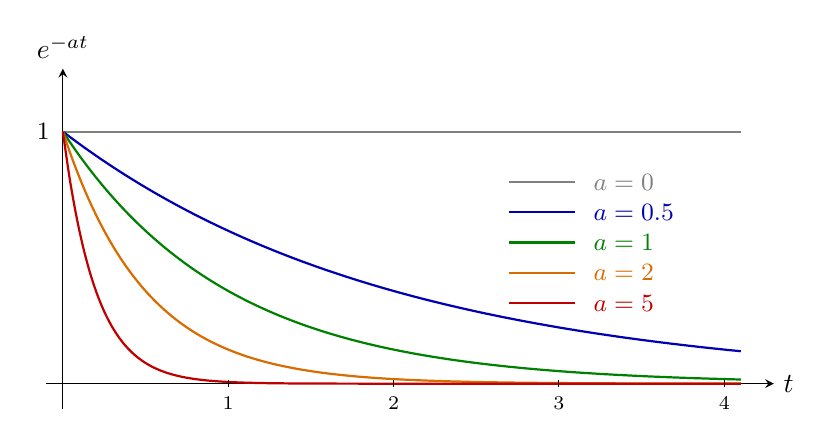
\begin{tikzpicture}[x=2.1cm,y=3.2cm,>=stealth]
  \draw[->] (-0.1,0) -- (4.3,0) node[right] {$t$};
  \draw[->] (0,-0.1) -- (0,1.25) node[above] {$e^{-at}$};
  \draw[dashed,gray] (0,1) -- (4.1,1);
  \node[left,font=\small] at (-0.02,1) {$1$};
  % a = 0: 恒为 1
  \draw[thick,gray] (0,1) -- (4.1,1);
  % a = 0.5, 1, 2, 5
  \draw[thick,blue!70!black, domain=0:4.1,samples=100,smooth] plot (\x,{exp(-0.5*\x)});
  \draw[thick,green!50!black,domain=0:4.1,samples=100,smooth] plot (\x,{exp(-1*\x)});
  \draw[thick,orange!85!black,domain=0:4.1,samples=100,smooth] plot (\x,{exp(-2*\x)});
  \draw[thick,red!75!black,  domain=0:4.1,samples=100,smooth] plot (\x,{exp(-5*\x)});
  % 图例（右上角，避免和曲线重叠）
  \foreach \y/\c/\lab in {0.80/gray/{a=0},0.68/blue!70!black/{a=0.5},0.56/green!50!black/{a=1},0.44/orange!85!black/{a=2},0.32/red!75!black/{a=5}} {
    \draw[thick,\c] (2.7,\y) -- (3.1,\y);
    \node[anchor=west,font=\small,\c] at (3.15,\y) {$\lab$};
  }
  \foreach \t in {1,2,3,4} { \draw (\t,0.015) -- (\t,-0.015) node[below,font=\scriptsize] {$\t$}; }
\end{tikzpicture}
\caption{衰减因子 $e^{-at}$（$t\ge0$）：$a=0$ 时恒为 $1$；$a$ 越大衰减越快，$a\to+\infty$ 时整条曲线被压向 $0$。}
\end{figure}
$a>0$ 时，这个因子还保证被积函数 $\frac{\sin t}{t}e^{-at}$ 在 $t\to+\infty$ 处快速衰减，积分一定收敛。

\textbf{第 2 步：对 $a$ 求导}（把求导放进积分号，$\frac{\partial}{\partial a}e^{-at}=-t\,e^{-at}$，正好把分母的 $t$ 消掉）：
\[
\frac{\d I}{\d a}=-\int_0^{+\infty}\sin t\;e^{-at}\d t
\]

\textbf{第 3 步：用欧拉公式}(Euler's formula) $\sin t=\dfrac{e^{jt}-e^{-jt}}{2j}$：
\begin{align*}
\frac{\d I}{\d a}
&=-\frac{1}{2j}\int_0^{+\infty}\bigl(e^{jt}-e^{-jt}\bigr)e^{-at}\d t\\
&=-\frac{1}{2j}\Bigl[\int_0^{+\infty}e^{-(a-j)t}\d t-\int_0^{+\infty}e^{-(a+j)t}\d t\Bigr]\\
&=-\frac{1}{2j}\Bigl[\frac{1}{a-j}-\frac{1}{a+j}\Bigr]
=-\frac{1}{2j}\cdot\frac{2j}{a^2+1}
=-\frac{1}{a^2+1}
\end{align*}
（这里 $a>0$ 保证 $e^{-(a\mp j)t}\to0$，积分才收敛。老师口头把负号并进括号里，写成 $\frac{1}{2j}\bigl[\frac{1}{a+j}-\frac{1}{a-j}\bigr]$，通分后分母 $a^2-j^2=a^2+1$、分子 $-2j$，结果一样；他说「积分学得好的一眼能看出」，并让大家课后自己验证这一步。）

\textbf{第 4 步：积分求 $I(a)$}：
\[
I(a)=-\arctan a+C
\]

\textbf{第 5 步：用 $a\to+\infty$ 定常数 $C$}。$a$ 很大时 $e^{-at}$ 把整个被积函数压成 $0$，所以 $I(+\infty)=0$：
\[
0=I(+\infty)=-\arctan(+\infty)+C=-\frac{\pi}{2}+C\ \Longrightarrow\ C=\frac{\pi}{2}
\]

\textbf{第 6 步：令 $a\to 0$}：
\[
I(0)=\int_0^{+\infty}\frac{\sin t}{t}\d t=-\arctan 0+\frac{\pi}{2}=\frac{\pi}{2}\qquad\blacksquare
\]

再由偶函数得 $\int_{-\infty}^{+\infty}\frac{\sin t}{t}\d t=2\cdot\frac\pi2=\pi$。

\emph{（补充：第 2 步「求导进积分号」和第 6 步「$a\to0^{+}$ 时 $I(a)\to I(0)$」严格来说需要论证收敛性，重转写里老师没有展开，他是直接把 $a=0$ 代入的，这一点是我看出来的，不是他说的。完整的论证见下面「收敛性与严格性」。）}\par\smallskip\textbf{老师在第 5 步的原话要点}：$a\to+\infty$ 时 $e^{-at}$ 趋于 0，被积函数每一点都趋于 0，所以 $I(+\infty)=0$；第 6 步「最后一步很有趣」：令 $a=0$，$e^{-0\cdot t}=1$，$I(0)$ 就是要求的积分。

\subsubsection*{收敛性与严格性（补充）}
\begin{note}
这一小节\textbf{不是老师课上讲的}，是我为了回答「证明里每一步为什么可以这样做」补的，用的是微积分里的标准做法，我自己核对过每一步。初学时可以先跳过，知道「证明里有这几个需要检查的地方」就够了。
\end{note}

证明里偷偷用了五件事，逐个检查。记 $F(t)=\displaystyle\int_t^{+\infty}\frac{\sin s}{s}\d s$（尾巴）。

\paragraph{（1）$\displaystyle\int_0^{+\infty}\frac{\sin t}{t}\d t$ 本身是收敛的。}
$t=0$ 附近没有问题：$\bigl|\frac{\sin t}{t}\bigr|\le1$。问题在 $t\to+\infty$。对 $R>1$ 做分部积分：
\[
\int_1^R\frac{\sin t}{t}\d t=\Bigl[-\frac{\cos t}{t}\Bigr]_1^R-\int_1^R\frac{\cos t}{t^2}\d t
=\cos1-\frac{\cos R}{R}-\int_1^R\frac{\cos t}{t^2}\d t .
\]
$R\to\infty$ 时，$\frac{\cos R}{R}\to0$；$\bigl|\frac{\cos t}{t^2}\bigr|\le\frac{1}{t^2}$，而 $\int_1^\infty\frac{1}{t^2}\d t$ 有限，所以最后一项也有极限。因此极限存在，积分收敛。

\textbf{但它只是「条件收敛」，不是「绝对收敛」}：在每个区间 $[k\pi,(k+1)\pi]$ 上，$\int\frac{|\sin t|}{t}\d t\ge\frac{1}{(k+1)\pi}\int|\sin t|\d t=\frac{2}{(k+1)\pi}$，把这些加起来像调和级数 $\sum\frac1k$ 一样发散，所以 $\int_0^\infty\frac{|\sin t|}{t}\d t=+\infty$。意思是：它收敛，靠的是正负波瓣相互抵消，而不是靠波瓣越来越小直至可以忽略。这个区别是下面第（5）条为什么要多费一点力气的原因。

\paragraph{（2）对 $a>0$，$I(a)$ 有意义。}
$\bigl|\frac{\sin t}{t}e^{-at}\bigr|\le e^{-at}$，而 $\int_0^\infty e^{-at}\d t=\frac1a$ 有限，所以绝对收敛。

\paragraph{（3）第 2 步「求导放进积分号」对 $a>0$ 成立。}
取任意 $a_0>0$。对所有 $a\ge a_0$：
\[
\Bigl|\frac{\partial}{\partial a}\Bigl(\frac{\sin t}{t}e^{-at}\Bigr)\Bigr|=|\sin t|\,e^{-at}\le e^{-a_0t},
\]
右边与 $a$ 无关，并且 $\int_0^\infty e^{-a_0t}\d t=\frac1{a_0}$ 有限。有这样一个「共同的、可积的上界」，微积分里「积分号下求导」的定理就成立。所以 $I'(a)=-\frac1{a^2+1}$ 对每个 $a>0$ 成立，再积分得 $I(a)=-\arctan a+C$（$a>0$，$C$ 是常数）。

\paragraph{（4）第 5 步 $I(+\infty)=0$ 的严格理由。}
$|I(a)|\le\int_0^\infty e^{-at}\d t=\frac1a\to0$（$a\to+\infty$），所以 $\lim_{a\to+\infty}I(a)=0$。代入 $I(a)=-\arctan a+C$，得 $0=-\frac\pi2+C$，$C=\frac\pi2$，即对所有 $a>0$：$I(a)=\frac\pi2-\arctan a$。

\paragraph{（5）第 6 步 $a\to0^{+}$ 时 $I(a)\to I(0)$：最需要小心的一步。}
我们已经知道 $I(a)=\frac\pi2-\arctan a$（$a>0$），所以 $\lim_{a\to0^+}I(a)=\frac\pi2$。要得到的是 $I(0)=\int_0^\infty\frac{\sin t}{t}\d t=\frac\pi2$，需要证明 $\lim_{a\to0^+}I(a)=I(0)$。

因为（1）说过 $\int\frac{\sin t}{t}\d t$ 只是条件收敛，不能用「被积函数有可积的上界，极限可以放进积分号」这类绝对收敛下的办法（这里找不到那个上界）。换一种办法：用尾巴 $F(t)$。

$F$ 连续，$F(0)=I(0)$，$F(t)\to0$（$t\to\infty$，因为是收敛积分的尾巴），$F'(t)=-\frac{\sin t}{t}$，并且 $F$ 有界，设 $|F|\le M$。于是对 $a>0$ 做分部积分：
\[
I(a)=\int_0^\infty\bigl(-F'(t)\bigr)e^{-at}\d t=F(0)-a\int_0^\infty F(t)\,e^{-at}\d t .
\]
（边界项：$t\to\infty$ 时 $F(t)e^{-at}\to0$。）接下来证明最后一项 $\to0$。任给 $\varepsilon>0$，选 $T$ 使得 $t>T$ 时 $|F(t)|<\varepsilon$，则
\[
\Bigl|a\int_0^\infty F(t)e^{-at}\d t\Bigr|
\le a\int_0^T M\d t+\varepsilon\cdot a\int_T^\infty e^{-at}\d t
\le aTM+\varepsilon .
\]
令 $a\to0^+$，右边 $\to\varepsilon$。$\varepsilon$ 是任意的，所以这一项趋于 $0$，于是 $I(a)\to F(0)=I(0)$。

\paragraph{合起来。}
$I(0)=\lim_{a\to0^+}I(a)=\lim_{a\to0^+}\bigl(\frac\pi2-\arctan a\bigr)=\frac\pi2$。证明因此是严格的。五个检查点里，（1）（5）是真正需要费力的，因为这个积分只是条件收敛；（2）（3）（4）都靠 $e^{-at}$ 的衰减，这也是老师「人为加一个因子」这一招有效的原因：它让积分在 $a>0$ 时变成绝对收敛，把棘手的部分推到了最后一步 $a\to0^+$。

%==================================================================
\section{基本的离散时间信号（书上第 15 页起）}

\subsection{单位脉冲序列 $\delta[n]$}
\[
\delta[n]=\begin{cases}1,&n=0\\0,&n\neq0\end{cases}
\]
书上叫它单位脉冲序列(unit impulse sequence)。老师的画法：横轴是 $n$，$n=0$ 处是 $1$，其他整数处都是 $0$。

\begin{figure}[H]
\centering
\begin{tikzpicture}[x=0.8cm,y=1.6cm,>=stealth]
  \draw[->] (-5.6,0) -- (5.9,0) node[right] {$n$};
  \draw[->] (0,-0.25) -- (0,1.5) node[above] {$\delta[n]$};
  % n=0: 高度 1 的竖线加实心圆
  \draw[very thick,blue!70!black] (0,0) -- (0,1);
  \fill[blue!70!black] (0,1) circle (2.5pt);
  % 其余整数：值为 0，画实心小圆
  \foreach \n in {-5,-4,-3,-2,-1,1,2,3,4,5} { \fill[blue!70!black] (\n,0) circle (2.5pt); }
  \node[left,font=\small] at (-0.1,1) {$1$};
  \foreach \n in {-4,-2,2,4} { \node[below,font=\scriptsize] at (\n,-0.07) {$\n$}; }
\end{tikzpicture}
\caption{单位脉冲序列 $\delta[n]$：只在 $n=0$ 处等于 $1$，其余整数处全为 $0$。与连续的 $\delta(t)$ 不同，这里每个点都有确定的有限值，没有「无穷大」。}
\end{figure}

\subsection{单位阶跃序列 $u[n]$}
\[
u[n]=\begin{cases}1,&n\ge0\\0,&n<0\end{cases}
\]
老师的画法：$n=0$ 处是 $1$，$n=1,2,\dots$ 也都是 $1$，一直延伸到右边；左边全是 $0$。

\begin{figure}[H]
\centering
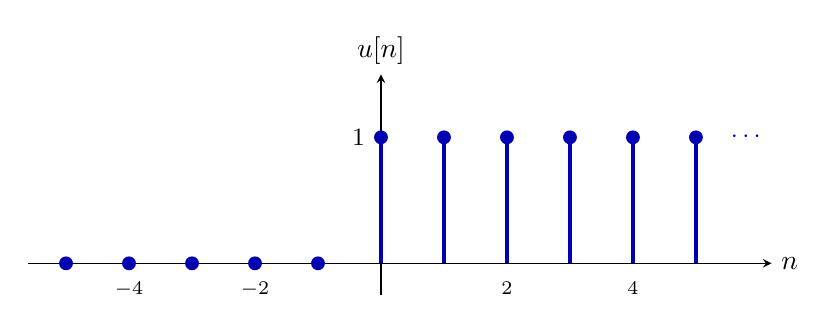
\begin{tikzpicture}[x=0.8cm,y=1.6cm,>=stealth]
  \draw[->] (-5.6,0) -- (6.2,0) node[right] {$n$};
  \draw[->] (0,-0.25) -- (0,1.5) node[above] {$u[n]$};
  % n>=0：高度 1
  \foreach \n in {0,1,2,3,4,5} {
    \draw[very thick,blue!70!black] (\n,0) -- (\n,1);
    \fill[blue!70!black] (\n,1) circle (2.5pt);
  }
  \node[right,font=\small,blue!70!black] at (5.4,1) {$\cdots$};
  % n<0：值为 0
  \foreach \n in {-5,-4,-3,-2,-1} { \fill[blue!70!black] (\n,0) circle (2.5pt); }
  \node[left,font=\small] at (-0.1,1) {$1$};
  \foreach \n in {-4,-2,2,4} { \node[below,font=\scriptsize] at (\n,-0.07) {$\n$}; }
\end{tikzpicture}
\caption{单位阶跃序列 $u[n]$：$n\ge0$ 时全为 $1$，$n<0$ 时全为 $0$。与连续的 $u(t)$ 不同，离散的 $u[0]$ 有明确的值 $1$，不需要「任取」。}
\end{figure}

\subsection{连续与离散的四个信号对照}
\begin{center}
\begin{tabular}{lcc}
\toprule
 & 连续（圆括号） & 离散（方括号）\\
\midrule
冲激 & $\delta(t)$：奇异，$t=0$ 处无穷大 & $\delta[n]$：普通，$n=0$ 处等于 1\\
阶跃 & $u(t)$：$t>0$ 为 1，$u(0)$ 任意 & $u[n]$：$n\ge0$ 为 1\\
\bottomrule
\end{tabular}
\end{center}
老师特别强调：\textbf{$\delta(t)$ 和 $\delta[n]$ 不是一回事}，常被搞混。$\delta[n]$ 是正常得不得了的信号（零处为 1，别处为 0）；$\delta(t)$ 是高中没学过的奇怪信号，第二章才会严格讲。区分的办法就是前面「圆括号连续、方括号离散」那条规则。

%==================================================================
\section{本节要记住的清单}
\begin{enumerate}[nosep]
\item $x(t)$ 连续，$x[n]$ 离散；没有 $x[t]$ 与 $x(n)$。
\item 偶 $+$ 奇分解：$x_e=\frac{x(t)+x(-t)}2$，$x_o=\frac{x(t)-x(-t)}2$，唯一。
\item 能量信号：$E<\infty$；功率信号：$P<\infty$。
\item $u(t)$：$t>0$ 为 1、$t<0$ 为 0，$u(0)$ 可任取；$\delta(t)=\frac{\d u}{\d t}$，$\int\delta=1$。
\item $\Sa(t)=\frac{\sin t}{t}$：偶函数，$\Sa(0)=1$，零点 $\pm k\pi$。
\item $\int_{-\infty}^{\infty}\Sa(t)\d t=\pi$；$\int_0^{\infty}\Sa(t)\d t=\frac\pi2$；$\int_{-\infty}^{\infty}\frac{\sin\omega t}{t}\d t=\pi\ (\omega>0)$。
\item $\delta[n]$、$u[n]$ 是离散里的对应物；$\delta[n]\neq\delta(t)$。
\end{enumerate}

\appendix
\section{附录：广义函数（generalized function）的说明}

\begin{note}
这个附录\textbf{不是老师课上讲的}：老师说严格的定义留到第二章。它是我为了解释正文里「$\delta(t)$ 不是普通函数」「$u(t)$ 在 $0$ 处不可导却有导数」「$u(0)$ 可以任取」这几句话而写的预习材料，内容是数学里的标准结论（分布论，distribution theory）。我没有查教材，如果第二章老师的讲法和这里不同，以老师和教材为准。
\end{note}

\subsection*{A.1 一句话主干}
\textbf{普通函数是「每个点给一个值」；广义函数不给点值，只规定「它作用在别的函数上，会得到一个什么数」。}$\delta(t)$ 就是这样的东西。下面一步一步讲，每一步只加一个新概念。

\subsection*{A.2 第一步：为什么普通函数这套说法不够用}
普通函数的想法是：给我一个 $t$，我告诉你函数值。$\delta(t)$ 想描述的是「一个极短、极强的冲击」，在 $t=0$ 处它的值是「无穷大」，而无穷大不是一个数，所以按「每点一个值」的办法，根本没法把 $\delta(t)$ 写成一个函数。

但这个冲击有一件事是\textbf{确定而有限}的：它对别的东西产生的\emph{总效果}。比如一个力的冲量（作用的总量），或者它去「抽取」另一个信号在某一点的值。数学家的办法是：\textbf{不去问它每点的值，只问它的总效果}。

\subsection*{A.3 第二步：测试函数（test function）——用来「试探」的工具}
先准备一类很乖的函数，叫\textbf{测试函数} $\varphi(t)$：
\begin{itemize}[nosep]
\item 无穷次可导（非常光滑，没有尖角、没有跳变）；
\item 在某个有限区间之外恒等于 $0$（像一个光滑的小山丘，两头平坦落地）。
\end{itemize}
它的作用像一把「探针」：用它去碰一碰广义函数，看反应。

\subsection*{A.4 第三步：广义函数 $=$ 一台「输入探针、输出一个数」的机器}
\textbf{广义函数}就是一台机器：你把一个测试函数 $\varphi$ 放进去，它吐出一个数，记作 $\langle T,\varphi\rangle$。（还要求这台机器是线性的、并且「探针变化很小则输出变化也很小」，初学可以先不管。）

\begin{remember}
\begin{itemize}[nosep]
\item $\delta$ 这台机器的规则：\textbf{输入 $\varphi$，输出 $\varphi$ 在 $0$ 点的值}：$\langle\delta,\varphi\rangle=\varphi(0)$。
\item 这正是课上「筛选性质」的来源：$\delta$ 像一个筛子，把 $\varphi$ 在 $0$ 处的值「筛」出来。
\item 普通函数 $f(t)$ 也能当一台机器：规则是 $\varphi\mapsto\int_{-\infty}^{+\infty}f(t)\varphi(t)\d t$。所以\textbf{普通函数是广义函数的特例}，广义函数是普通函数的推广。
\end{itemize}
\end{remember}
$\delta$ 之所以叫\textbf{奇异}的（singular），就是因为\emph{没有}任何普通函数能产生「$\varphi\mapsto\varphi(0)$」这台机器。

\subsection*{A.5 第四步：为什么说 $\delta$ 是窄脉冲的「极限」}
正文里用宽 $\Delta$、高 $1/\Delta$ 的矩形脉冲 $\delta_\Delta(t)$ 来想象 $\delta(t)$。现在可以说清楚这个极限是什么意思了：
\[
\langle\delta_\Delta,\varphi\rangle=\frac{1}{\Delta}\int_0^{\Delta}\varphi(t)\d t
\ \xrightarrow{\ \Delta\to0\ }\ \varphi(0)=\langle\delta,\varphi\rangle .
\]
（$\Delta$ 很小时，$\varphi$ 在 $(0,\Delta)$ 上几乎就是常数 $\varphi(0)$，取平均就得到 $\varphi(0)$。）

这叫\textbf{弱收敛}：不是「每一点的函数值收敛」，而是「放进每一个探针，输出都收敛」。逐点看，$\delta_\Delta(0)$ 是 $1/\Delta\to\infty$ 的，根本不收敛；但用探针一试，它收敛得很好。这也解释了为什么\textbf{换成三角形、高斯曲线等别的窄脉冲，只要面积是 $1$、宽度趋于 $0$，结果都一样}：探针看到的只是「面积 $1$、集中在 $0$」这件事。

\subsection*{A.5 第五步：广义导数——解释 $\delta(t)=\dfrac{\d u(t)}{\d t}$}
先看普通函数。对光滑的 $f$，用分部积分（探针在两头为 $0$，边界项消失）：
\[
\int f'(t)\varphi(t)\d t=-\int f(t)\varphi'(t)\d t .
\]
也就是说：\textbf{把导数从 $f$ 身上「转移」到探针 $\varphi$ 身上，只多一个负号}。右边的写法即使 $f$ 本身不可导也有意义（只要 $f$ 能积分）。于是数学家\textbf{规定}：
\[
\langle T',\varphi\rangle:=-\langle T,\varphi'\rangle
\]
这就是\textbf{广义导数}的定义。好处是：\textbf{任何广义函数都能求导，而且可以求无限次}。

现在算 $u(t)$ 的广义导数（这一步就是课件那句「不能作为定义式」背后的严格版本）：
\begin{align*}
\langle u',\varphi\rangle
&=-\langle u,\varphi'\rangle=-\int_{-\infty}^{+\infty}u(t)\varphi'(t)\d t
=-\int_{0}^{+\infty}\varphi'(t)\d t\\
&=-\bigl[\varphi(+\infty)-\varphi(0)\bigr]=\varphi(0)=\langle\delta,\varphi\rangle .
\end{align*}
（用到了 $u(t)$ 只在 $t>0$ 取 $1$，以及 $\varphi$ 在远处为 $0$。）所以 $u'=\delta$ \textbf{在广义函数的意义下严格成立}，不是什么「工程上的近似」。课件说「不能作为定义式」是因为：这个等式要先有「广义导数」这套规则才有意义，而 $\delta$ 的定义本身（A.4 的筛选规则）不依赖它。

用同样的办法：
\begin{itemize}[nosep]
\item \textbf{冲激偶}（doublet）$\delta'(t)$：$\langle\delta',\varphi\rangle=-\langle\delta,\varphi'\rangle=-\varphi'(0)$，它「筛出」的是探针在 $0$ 处的\textbf{导数}（带负号）。
\item 一个信号在 $t_0$ 处有向上跳变 $A$，它的广义导数 $=$ 普通导数（$t\neq t_0$ 处的斜率）$+\ A\,\delta(t-t_0)$。正文里的 $5\delta(t)$、$\delta(t-2)$ 都是它的特例。
\end{itemize}

\subsection*{A.6 第六步：回答老师留的悬念——为什么 $u(0)$ 可以取任意值}
广义函数是靠「积分的结果」来识别的。如果两个普通函数只在\textbf{一个点（或有限个点）}上不同，那么对任何探针 $\varphi$，$\int f\varphi\d t$ 的结果完全一样，因为一个点的「宽度」是零，对积分没有贡献。所以这两个函数产生的是\textbf{同一台机器}，也就是同一个广义函数。

$u(0)$ 取 $0$、$\tfrac12$、$1$ 甚至 $-1$，只改变了 $t=0$ 这一个点的值，机器完全不变，所以信号与系统里它是「可以任取」的。\emph{（这是我的解释；老师说第二章会讲，我猜他讲的就是这件事，但没有证据，不能当成老师的原话。）}

反过来，这也说明了一个重要的限制：\textbf{广义函数没有「某一点的值」这回事}。问「$\delta(0)$ 等于几」本身就是没意义的问题，正文里写的「$t=0$ 处为 $+\infty$」只是帮助想象的说法。

\subsection*{A.7 几条要小心的限制}
\begin{itemize}
\item \textbf{没有点值}：见上，不能问 $\delta(t_0)$ 是多少。
\item \textbf{不能随便相乘}：$\delta(t)\cdot\delta(t)$ 没有意义（两个广义函数一般不能相乘）。但「广义函数 $\times$ 光滑函数」是可以的，比如 $f(t)\delta(t)=f(0)\delta(t)$（$f$ 光滑），这是筛选性质的另一种写法。
\item \textbf{「连续、间断」这类说法用不上}：这是逐点的概念，而广义函数不逐点定义。
\end{itemize}

\subsection*{A.8 小结}
\begin{center}
\begin{tabular}{p{0.2\textwidth}p{0.36\textwidth}p{0.3\textwidth}}
\toprule
 & 普通函数 & 广义函数 \\
\midrule
怎么定义 & 每个点给一个值 & 作用在探针 $\varphi$ 上给一个数 \\
$\delta$ 怎么描述 & 无法描述（$+\infty$ 不是数） & $\varphi\mapsto\varphi(0)$ \\
导数 & 要求连续、可导 & 转移到探针上，总是存在，可无限次求导 \\
单点的值 & 有，且影响函数本身 & 没有，改一个点不影响 \\
\bottomrule
\end{tabular}
\end{center}
所以：\textbf{$\delta(t)=\frac{\d u}{\d t}$ 是严格成立的，只不过是在广义函数的意义下；$\delta$ 的「无穷大」是想象的拐杖，真正的定义是筛选性质。}

\end{document}
